\documentclass[conference]{IEEEtran}
\IEEEoverridecommandlockouts
% The preceding line is only needed to identify funding in the first footnote. If that is unneeded, please comment it out.
\usepackage{cite}
\usepackage{amsmath,amssymb,amsfonts}
\usepackage{algorithmic}
\usepackage{graphicx}
\usepackage{textcomp}
\usepackage{xcolor}
\def\BibTeX{{\rm B\kern-.05em{\sc i\kern-.025em b}\kern-.08em
    T\kern-.1667em\lower.7ex\hbox{E}\kern-.125emX}}
\begin{document}

\title{CS 6200 Information Retrieval Final Project\\
Report\\
{\footnotesize Spring 2019 \textemdash Professor Rukmini Vijaykumar}
}

\author{\IEEEauthorblockN{Brian Desnoyers}
\IEEEauthorblockA{\textit{Khoury College of Computer Sciences} \\
\textit{Northeastern University}\\
Boston, MA, U.S.A. \\
bdesnoy@ccs.neu.edu}
\and
\IEEEauthorblockN{John Goodacre}
\IEEEauthorblockA{\textit{Khoury College of Computer Sciences} \\
\textit{Northeastern University}\\
Boston, MA, U.S.A. \\
goodacre.j@husky.neu.edu}
\and
\IEEEauthorblockN{Akshay Kulkarni}
\IEEEauthorblockA{\textit{Khoury College of Computer Sciences} \\
\textit{Northeastern University}\\
Boston, MA, U.S.A. \\
kulkarni.akshay@husky.neu.edu}
}

\maketitle

\section{Introduction}
This project explores the development and evaluation of several search engines for a provided test collection of scholarly journal abstracts. Baseline systems were improved via query enhancement techniques, such as word embedding query expansion and stemming. A snippet generation and spelling error correction model were also developed to improve the baseline retrieval systems.
\\\\
Team member contributions (in addition to the homework retrieval models) are listed below:
\begin{itemize}
\item Brian Desnoyers
\begin{itemize}
\item Baseline Query Likelihood Model (JM smoothed)
\item Baseline Query Likelihood Model (Dirichlet Smoothed)
\item Word Embedding-Based Query Expansion
\item Task 3- Stopping and Stemming
\item Snippet Generation and Query Term Highlighting
\item Phase 3- Evaluation
\item Relevant Sections of Readme Documentation
\item Relevant Sections of Final Report
\end{itemize}
\item John Goodacre
\begin{itemize}
\item Task 3- Stopping
\item Relevant Sections of Readme Documentation
\item Relevant Sections of Final Report
\end{itemize}
\item Akshay Kulkarni
\begin{itemize}
\item Vector-Space Term Frequency–Inverse Document Frequency model 
\item Rocchio Algorithm for Relevance Feedback w/ Vector-Space Model
\item Relevant Sections of Readme Documentation
\item Relevant Sections of Final Report
\end{itemize}
\end{itemize}

\section{Background}
% AKA Techniques to be used and justification, Literature and resources
\subsection{Dataset}
This project utilizes a dataset consisting of 3024 abstracts from the Communications of the ACM (CACM) published between 1958 and 1979 \cite{croftsearch}. In addition, the DBLP Computer Science Bibliography was utilized for generating models used for query expansion. This database is a collection citation information from computer science journal articles \cite{ley2002dblp}.
\subsection{Baseline Models}
This project involves the development of several information retrieval systems, with an evaluation and comparison of their performance in terms of retrieval effectiveness. This involves four baseline models.
\\\\
The first baseline model is a Best Matching 25 (BM25) ranking \cite{robertson1995okapi}, which expands the binary independence model to incorporate term weights for both queries and documents. This method attempts to estimate the probability that a particular document is relevant, assuming that terms are independent given document relevance \cite{yu1975precision}, similar to a Na\"ive Bayes classifier. The BM25 algorithm can also be used in the absence of relevance information, however. The BM25 ranking algorithm is thus a probabilistic model.
\\\\
The second and third baseline models are both query likelihood models which compute the probability of a query based on the language model for each document. These models use simple unigram language models for each document. Because it is unlikely that all relevant documents will contain the query terms, in order for their language models to generate those terms, smoothing must be used. One of these models uses Jelinek-Mercer (JM) smoothing, which uses a probability from a collection-wide language model to adjust the probability cite{croftsearch}. The weight of this term is adjusted by a parameter $\lambda$, which increases the smoothing effect. Thus small values, such as $0.1$ tend to work well for shorter queries, while larger values, such as $0.7$ tend to work better for longer queries \cite{croftsearch}. The other model uses Dirichlet Smoothing /cite{croftsearch}. which instead uses a parameter $\mu$, which increases the weighting of documents with more matching terms \cite{croftsearch}. Dirichlet Smoothing typically performs better than JM smoothing on smaller queries, and typical values for $\mu$ are between $1000$ and $2000$.
\\\\
The fourth (an extra) baseline model is a term frequency–inverse document frequency (tf-idf) vector space model \cite{salton1988term}. This model involves computing distances between document and query vectors, through metrics such as cosine distance, which was utilized for this project. These vectors are computed based on the tf-idf values for each term within the vocabulary, which is product of the term frequency within the document and the reciprocal document frequency of the term \cite{salton1988term}. The Tf-Idf Vector Space model has been implemented by computing ranking scores based on dot product of cosine weights of tf-idf vectors computed from a document index, In order to reduce the impact of frequent terms, log transformation with laplace smoothing was applied to raw term frequencies. Additionally Rocchio relevance feedback method (Rocchio's algorithm) was incorporated into the Vector Space model as a query modification method using the relevance information provided, which transforms the query term weights in the query vector by adding a component based on the average of weights in the relevant documents and negating by a component based on the average weight in the non-relevant documents.
\\\\
The final baseline model is Lucene, which is an open-source indexing and searching tool \cite{bialecki2012apache}, and is used within common search engine implementations, such as Apache Solr \cite{grainger2014solr} and Elasticsearch \cite{divya2013elasticsearch}. Lucene uses its own scoring function which is based on tf-idf \cite{bialecki2012apache}.

\subsection{Query Enhancement}
\subsubsection{Query Expansion}
Query expansion is a method used to improve retrieval system performance and relevance by adding additional terms to a query \cite{efthimiadis1996query}. Several methods for query expansion exist, including pseudo-relevance feedback and word embedding-based query expansion. Pseudo-relevance feedback uses highly ranked documents to select new terms for query expansion and has been shown to be effective both with and without improvements, such as a term proximity heuristic for selecting expansion terms near query terms \cite{lv2010positional}. Another modern query expansion technique involves the use of word embeddings, which are commonly used in natural language processing. Word embeddings map co-occurance information to a lower dimensional space, often using a skip-gram or continuous bag of words model. Query expansion terms can be identified by finding nearest neighbors to query terms via these models \cite{diaz2016query}.
\subsubsection{Stopping}
Stopping is a technique used to filter out specific words, known as stop words. Ideally these stop words will be common across many documents in the collection and thus have limited semantic meaning or impact on document relevance. Words might carry little meaning from a frequency (or information theoretic) point of view, or alternatively from a conceptual (or linguistic) point of view. Words that occur in many of the documents in the collection carry little meaning from a frequency point of view, because a search for documents that contain that word will retrieve many of the documents in the collection. By removing the very frequent words, the document rankings will not be affected that much. While these stop words can be removed at index time, but are often used only at query time as this allows for more flexibility during search. Stop word removal on the basis of frequency can be done easily by removing the words with the highest
frequencies in the document collection. As a result of stopping the most 200-300 frequent words, indexes may be between 30\% and 50\% smaller \cite{djoerd2001statistical}.
\subsubsection{Stemming}
Stemming is the process of reducing all words with the same root (or, if prefixes are left untouched, the same stem) to a common form, usually by stripping each word of its derivational
and inflectional suffixes. There are various stemming strategies developed for different purposes\cite{Lovins1968DevelopmentOA}. Some stemming algorithms utilize a stem dictionary and others a suffix list. Many stemming algorithms, designed to improve IR performance and document relevance, do not use
a stem dictionary, but an explicit list of suffixes, and the criteria for removing suffixes. Stemmers of the popular stemmer family, the Porter stemmers, have adopted this approach \cite{airio2006word}.
\\\\
\subsection{Snippet Generation and Highlighting}
A classical approach for snippet generation is extractive summarization using an extension of Luhn's Algorithm \cite{luhn1958automatic}. This algorithm involves the identification of key phrases within sentences containing query terms. The query terms identified within these key phrases can be highlighted to the user via the search engine interface.

\section{Implementation and Discussion}
% Design choices and justification
\subsection{Baseline Model Implementation}
The baseline models will be implemented in Python. The tf-idf vector space model was implemented by computing ranking scores based on cosine distance of tf-idf vectors computed based on a document index. This utilized a vocabulary generated from the index, with Laplace smoothing. Similarly, the query liklihood and BM25 baselines were implemented in Python. The final Lucene-based model was developed using PyLucene \cite{vajda2005pulling}.

\subsection{Query Enhancement}
Query expansion was performed via pseudo-relevance feedback and Word2vec-trained \cite{mikolov2015computing} word embeddings. For pseudo-relevance feedback, $6$ query terms were selected based on the $10$ top ranked documents to find the expansion terms. Due to the limited size of the training set, a set of word embeddings from about three million article titles from the DBLP Computer Science Bibliography. This utilized a continuous bag of words model with a vector size of $100$ and window size of $10$ for use during training, as these are common parameters for these purposes \cite{mikolov2013distributed}. The Gensim library was used to perform initial processing of these word embeddings \cite{rehurek_lrec}. Stopping utilized the provided project stop list. Stemming utilized the provided query and document files.

\subsection{Snippet Generation and Highlighting}
Snippet generation was performed via extractive summarization using an extension of Luhn's Algorithm. Sentences were ranked based on a computed significance factor, which is the number of query terms within the key phrase divided by the total number of words in the key phrase. Initial query terms were extracted and highlighted within the terminal output (\verb|\033[1m term \033[0m|).

\subsection{Combining Approaches}
To combine approaches, a final run was performed that combines stopping with the word embedding query expansion technique.

\subsection{Extra Credit}
A spelling error interface was implemented. This interface used a unigram language model trained via the dataset which was used in conjunction with a noisy channel model to provide up to $6$ suggestions with the highest probability for each query word not in the index. As shown in Figure \ref{fig:spelling}, this spelling corrector also found similar words such as singular/plural forms when one wasn't in the index.

\begin{figure*}
  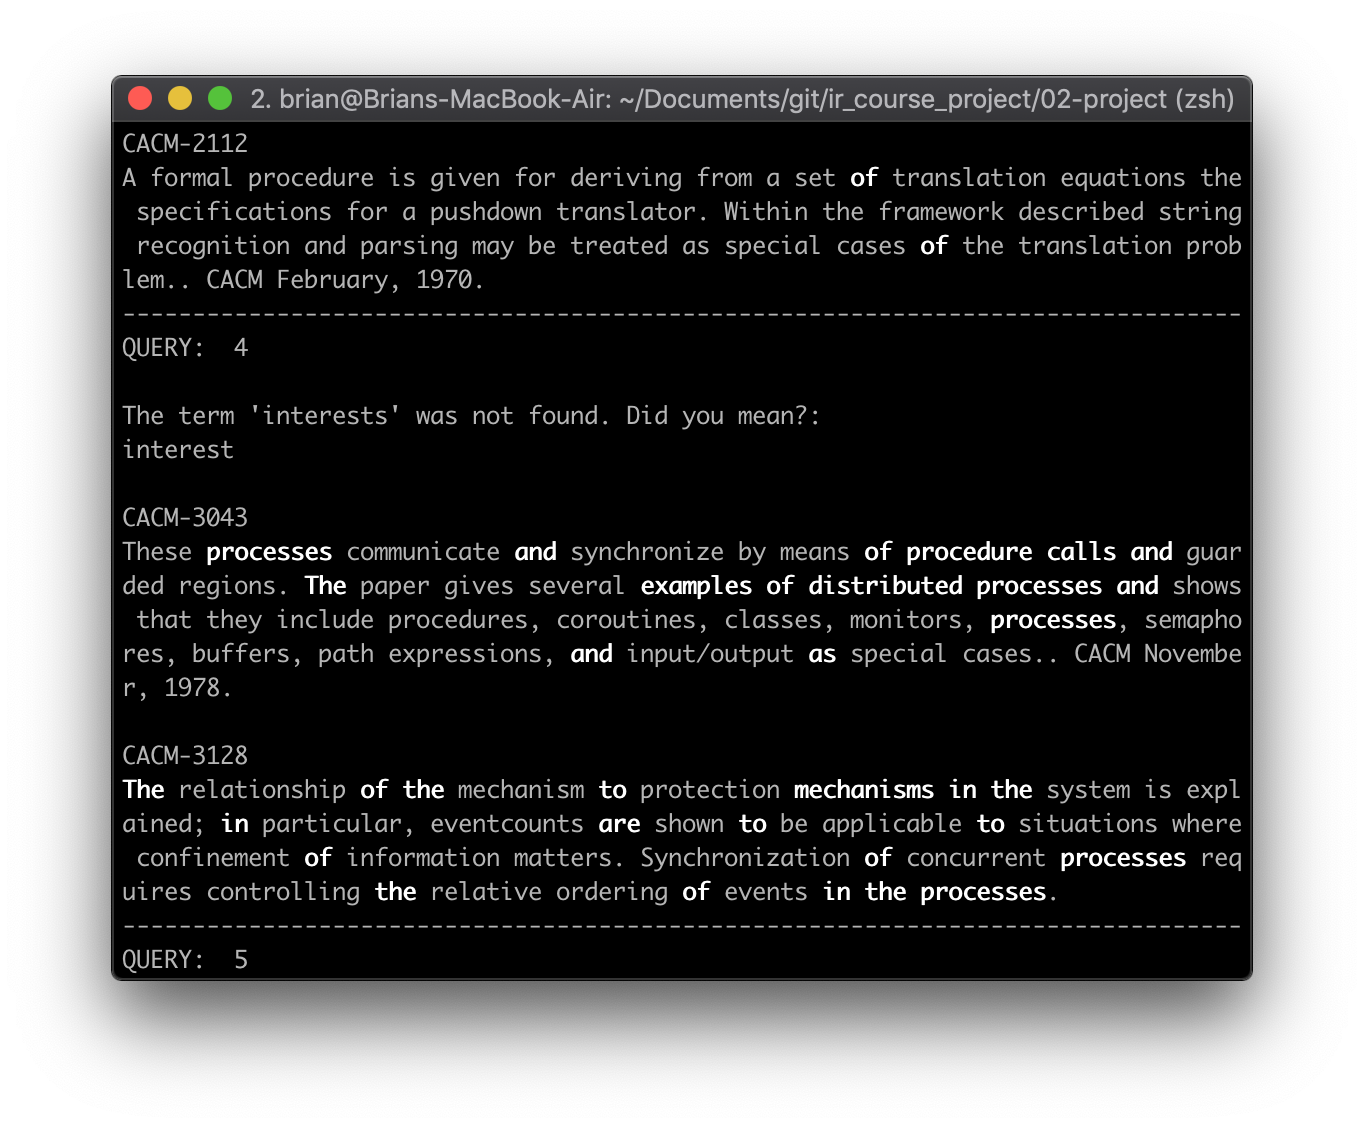
\includegraphics[width=\textwidth]{suggestion}
  \caption{An example suggestion from the spelling corrector. In this example, since query expansion was not used, a suggestion was made to change a plural form to the singlular.}
  \label{fig:spelling}
\end{figure*}

\subsection{Query-by-Query Analysis}
Looking at, for example, the query "What articles exist which deal with TSS (Time Sharing System), an operating system for IBM computers?," the top result for BM25 and the QLM discuss storage structures which is not relevant.  The top document for the Lucene model discusses a computer sharing system. This result occurs even when stopping is applied to the BM25 model. When stopping is added to Lucene, however, the first result is about a time sharing system. In this single query-by-query example, the stopping seems to have a more positive impact on the Lucene model. This is discussed and analyzed in more detail across the dataset using evaluation metrics as described in the Results section of this document.
\\\\
Query-by-query analysis for the stemming results is included in the Results section of this document.

\section{Results}
The summary of results across all runs is shown in Table \ref{fig:results}. This includes mean average precision (MAP), mean reciprocal rank (MRR), precision at $k$ for $k=5$ and $k=20$ (P@5, P@20), overall precision (for all 100 documents), and overall recall (for all 100 documents). Complete query-by-query results are included with this submission as described in \verb|Readme.txt| (files named \verb|results_*.txt|). Similarly, full tables for all evaluation metrics are included with this submission as described in \verb|Readme.txt| (files named \verb|eval_*.txt|). For the stopping there was 77.4\% overlap for the BM25 results and 84.9\% overlap for the Lucene results.

\begin{figure*}
  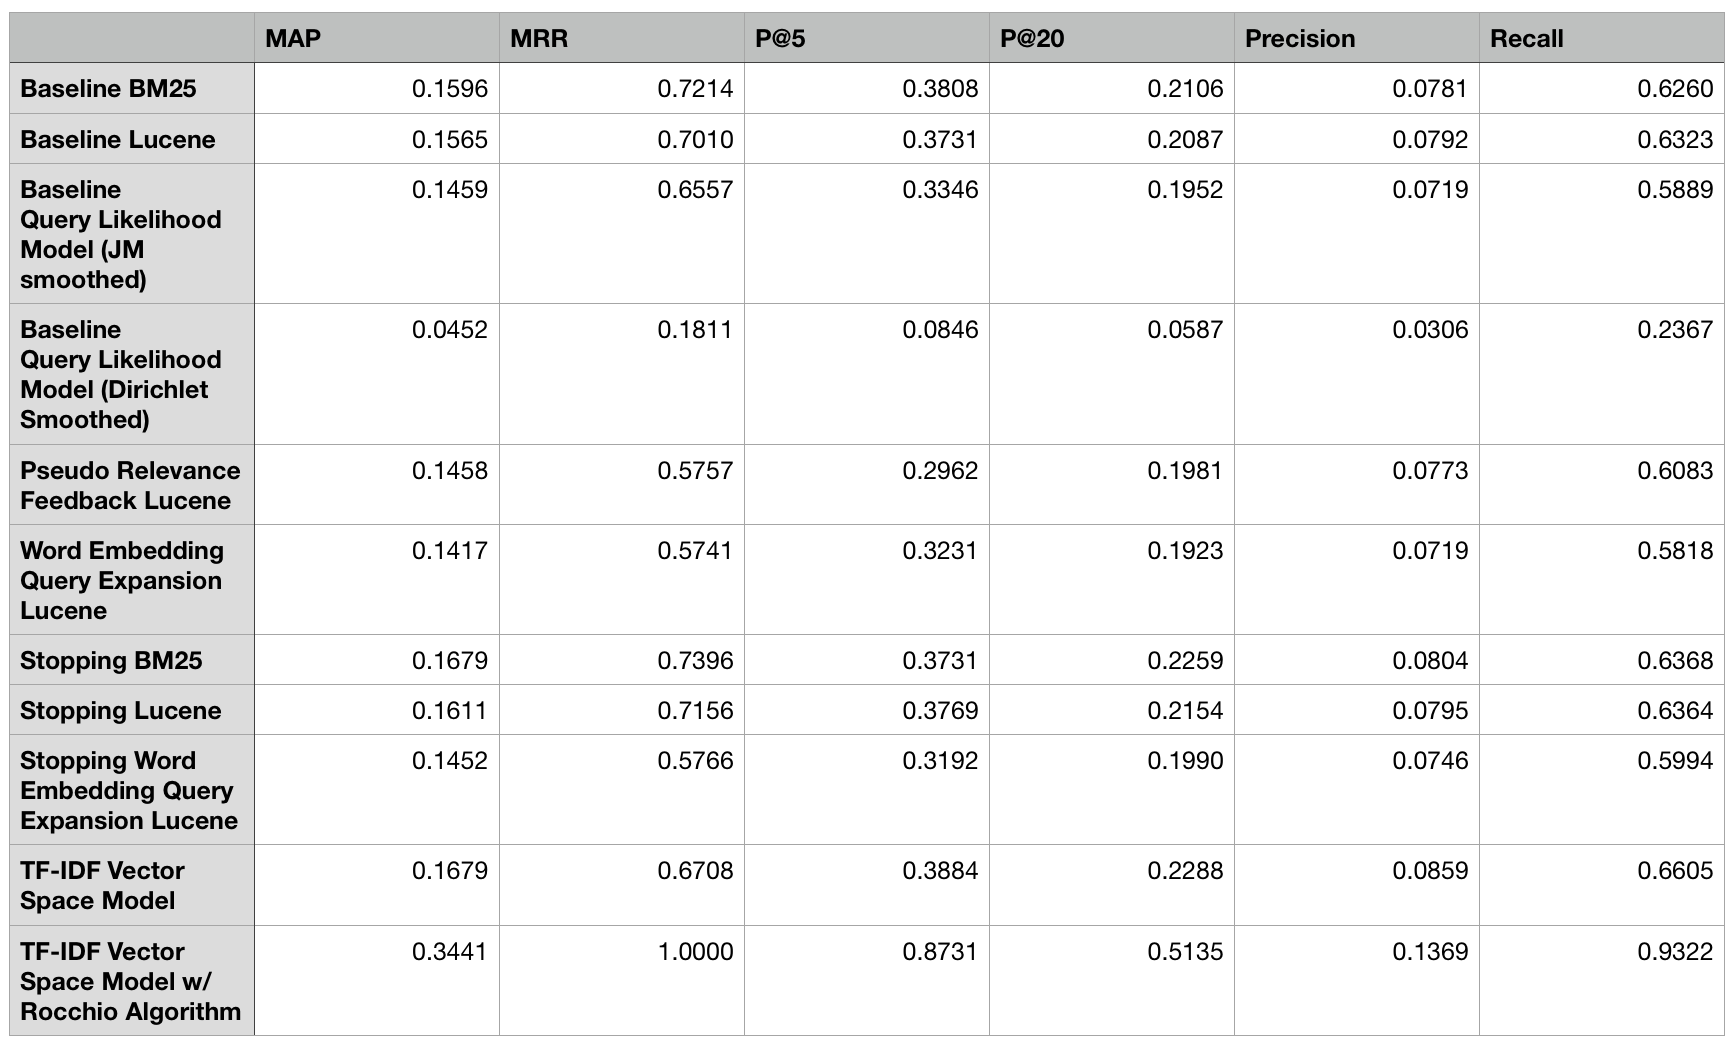
\includegraphics[width=\textwidth]{results_summary_table}
  \caption{A summary of the result table across all main runs.}
  \label{fig:results}
\end{figure*}

Results are interpreted within the Conclusion section of this document.

\subsection{Stemming Results}
While the stemming results could not be directly compared, they yielded highly similar results that appeared to be relevant qualitatively. For example, for the first query, "portabl oper system," the top results from both systems were extremely similar, which was not the case for results from the previous runs. This is likely not only due to the stemming, but also because of the fact that the queries used for the stemming sources were much more succinct. This demonstrates that many of the models used, specifically the BM25 and standard Lucene models, may work better for concise keyword queries, rather than prose. Similar results occurred for the second query "code optim for space effici", and the top hits referring to space efficient code, such as the top result about indirect threaded code (\verb|CACM-2748.html|).

\section{Conclusion}
From these result tables, it is clear that the TF-IDF model using Rocchio relevance feedback performed best, however, it should be noted that it had ground-truth relevance information available. This therefore likely artificially inflated the results, as seen by the mean reciprocal rank value of $1.0$. While the standard TF-IDF vector space model performed very well in comparison to other systems (e.g. its MAP was similar to the BM25 algorithm after stopping), its efficiency made its use significantly less desirable. One area for future work is to improve the tf-idf vector space model as it had limited performance during this assignment, taking almost an hour to run through all the queries.
\\\\
These tables also show that the impacts of enhancements, such as query expansion, may have been limited by the non-succinctness of the queries used. While results during expansion, especially for the word embedding-based query expansion, were able to find similar terms (e.g. system to systems), they also found synonyms for non-stopwords that should be removed. As a result, these measures appeared to only moderately improve performance.
\\\\
Despite the traditional improvement of Dirichlet smoothing over JM smoothing for a query likelihood model \cite{croftsearch}, the JM smoothed model appeared to significantly outperform the other model, likely due to the length of the queries \cite{croftsearch}.
\\\\
Similarly the BM25 model seemed to slightly perform the Lucene-based model based on its MAP, MRR, and P@5 values.

%Conclusions and outlook: state your findings, observations and analyses of the results. Which system do you think works best? Why? For “outlook”: write a few sentences stating what you would envision doing to improve your project, what other features you would choose to incorporate.

\bibliography{paper-sources}{}
\bibliographystyle{ieeetran}

\end{document}
